% presentaciones/sesion08-cap08/sesion08.tex
% Sesión 8 — Capítulo 8: Figuras participantes en la decisión digital
% Laboratorio: Gestión de datos, comportamiento y perfiles del consumidor digital
% Lic. en Mercadotecnia Digital · ESCA Unidad Santo Tomás · IPN
% Fuente de contenido: libro-consumidor-digital/partes/parte2/cap08.tex
% Figuras reutilizadas del libro (TikZ y MATLAB) sin copiarlas: ver \graphicspath y \input.
\documentclass[aspectratio=169,xcolor=dvipsnames]{beamer}
\usetheme{Berlin}

%----------------------------------------------------------------------------------------
%   PALETA INSTITUCIONAL IPN (Manual de Identidad Gráfica, Pantone 222C)
%----------------------------------------------------------------------------------------
\usepackage[dvipsnames,svgnames,x11names]{xcolor}
\definecolor{IPNguinda}{HTML}{6F1D46}       % Pantone 222C oficial — color primario
\definecolor{IPNguindaOsc}{HTML}{45102C}    % sombra / paleta secundaria
\definecolor{IPNguindaClara}{HTML}{F4E9EF}  % fondo de bloques normales
\definecolor{IPNdorado}{HTML}{B8975A}       % dorado — SOLO enlaces y detalles del cierre
\definecolor{IPNterracota}{HTML}{9C5B44}    % alertblock
\definecolor{IPNterracotaClara}{HTML}{F6ECE6}
\definecolor{IPNbronce}{HTML}{8C6B3F}       % exampleblock
\definecolor{IPNbronceClaro}{HTML}{F5F0E3}
\definecolor{IPNgris}{HTML}{58595B}         % texto secundario / notas

% Alias con los nombres de config/colores.tex del libro, para que las figuras
% TikZ del libro se puedan \input sin modificarlas
\colorlet{guindaIPN}{IPNguinda}
\colorlet{guindaIPNOsc}{IPNguindaOsc}
\colorlet{guindaIPNClara}{IPNguindaClara}
\colorlet{doradoIPN}{IPNdorado}
\colorlet{bronceIPN}{IPNbronce}
\colorlet{bronceIPNClaro}{IPNbronceClaro}
\colorlet{grisIPN}{IPNgris}
\colorlet{terracotaIPN}{IPNterracota}
\colorlet{terracotaIPNClara}{IPNterracotaClara}
\definecolor{colorLaboratorio}{HTML}{1B6E7A}

\setbeamercolor{palette primary}{bg=IPNguinda,fg=white}
\setbeamercolor{palette secondary}{bg=IPNguindaOsc,fg=white}
\setbeamercolor{palette tertiary}{bg=IPNguindaOsc,fg=white}
\setbeamercolor{palette quaternary}{bg=IPNguinda,fg=white}
\setbeamercolor{structure}{fg=IPNguinda}
\setbeamercolor{title}{bg=IPNguinda,fg=white}
\setbeamercolor{frametitle}{bg=IPNguinda,fg=white}
\setbeamercolor{block title}{bg=IPNguinda,fg=white}
\setbeamercolor{block body}{bg=IPNguindaClara,fg=black}
\setbeamercolor{block title alerted}{bg=IPNterracota,fg=white}
\setbeamercolor{block body alerted}{bg=IPNterracotaClara,fg=black}
\setbeamercolor{block title example}{bg=IPNbronce,fg=white}
\setbeamercolor{block body example}{bg=IPNbronceClaro,fg=black}
\setbeamercolor{alerted text}{fg=IPNterracota}
\setbeamercolor{item}{fg=IPNguinda}
\setbeamercolor{section in toc}{fg=IPNguinda}
\setbeamercolor{footline}{bg=IPNguindaOsc,fg=white}

\usepackage[spanish,es-noshorthands,es-nodecimaldot]{babel}
\usepackage{csquotes}
\usepackage{hyperref}
\usepackage{graphicx}
\usepackage{booktabs}
\usepackage{array}
\usepackage{amsmath}
\setbeamertemplate{caption}[numbered]
\usepackage{xurl}
\usepackage{adjustbox}
\usepackage{tikz}
\usetikzlibrary{arrows.meta,positioning,shapes.geometric}
\usepackage{pgfplots}
\pgfplotsset{compat=1.18}

\graphicspath{{Figures/}{../../libro-consumidor-digital/figuras/matlab/}}
\newcommand{\figtikz}[1]{../../libro-consumidor-digital/figuras/tikz/#1}
\newcommand{\fuente}[1]{{\tiny\color{IPNgris}Fuente: #1}}

\hypersetup{
    colorlinks=true,
    linkcolor=IPNdorado,
    filecolor=IPNguinda,
    urlcolor=IPNguinda,
    citecolor=IPNguinda,
    pdftitle={Sesion 8 - Figuras participantes},
    pdfauthor={Dr. Aboud Barsekh-Onji},
}

%----------------------------------------------------------------------------------------
%   CODE LISTINGS — sintaxis ESTÁNDAR del lenguaje
%----------------------------------------------------------------------------------------
\usepackage{listings}
\definecolor{backcolour}{rgb}{0.97,0.97,0.99}
\definecolor{codegreen}{rgb}{0,0.6,0}

\lstdefinestyle{MATLABStyle}{
  language=Matlab,
  basicstyle=\ttfamily\scriptsize,
  keywordstyle=\color{blue}\bfseries,
  commentstyle=\color{codegreen},
  stringstyle=\color{violet},
  breaklines=true,
  numbers=left,
  numbersep=5pt,
  frame=lines,
  backgroundcolor=\color{backcolour}
}
\lstset{style=MATLABStyle}

%----------------------------------------------------------------------------------------
%   TITLE CONFIGURATION
%----------------------------------------------------------------------------------------
\logo{
\includegraphics[height=0.75cm]{ipn-escudo.png}}
\title[Sesión 8 · Figuras participantes]{Figuras participantes en la decisión digital}
\subtitle{Sesión 8 · Unidad II — Capítulo 8}
\author{Dr. Aboud Barsekh-Onji}
\institute[IPN]{
    Instituto Politécnico Nacional \\
    \small ESCA Unidad Santo Tomás · Lic. en Mercadotecnia Digital \\
    \footnotesize Laboratorio: Gestión de datos, comportamiento y perfiles del consumidor digital
}
\date{\today}

%----------------------------------------------------------------------------------------
%   AUTO AGENDA AT EACH SECTION
%----------------------------------------------------------------------------------------
\AtBeginSection[]{
  \begin{frame}{Agenda}
    \tableofcontents[currentsection]
  \end{frame}
}



\begin{document}

\begin{frame}
    \titlepage
    \vspace{-4pt}
    \begin{center}
        {\tiny\color{IPNgris} ORCID: \href{https://orcid.org/0009-0004-5440-8092}{0009-0004-5440-8092}}
    \end{center}
\end{frame}

%------------------------------------------------
\section{Encuadre}
%------------------------------------------------

\begin{frame}{Ficha de la sesión}
\begin{columns}[T]
  \column{0.52\textwidth}
  \begin{block}{Unidad II}
    \small Proceso de toma de decisión de compra digital
  \end{block}
  \begin{block}{Tema del programa (2.3 Figuras participantes)}
    \scriptsize
    \begin{itemize}
      \item[2.3.1] Consumidor / Usuario / \textit{Buyer persona} / Prosumidor
      \item[2.3.2] Influenciador / \textit{Influencer}
      \item[2.3.3] Decisor \quad [2.3.4] Comprador \quad [2.3.5] Evaluador
    \end{itemize}
  \end{block}
  \column{0.44\textwidth}
  \begin{block}{Carga horaria}
    \small Teoría 3.0 h · Práctica 2.0 h\\ Aprendizaje autónomo 1.0 h
  \end{block}
  \begin{exampleblock}{Competencia de la unidad}
    \small Examina el proceso de toma de decisiones de compra del consumidor digital a partir de su recorrido y figuras participantes.
  \end{exampleblock}
\end{columns}
\end{frame}

\begin{frame}{Al terminar la sesión podrás\ldots}
\begin{enumerate}
  \item \textbf{Distinguir} siete figuras de la decisión de compra y reconocer que una persona puede reunir varias.
  \vspace{4pt}
  \item \textbf{Explicar} el origen y los límites del \textit{buyer persona}.
  \vspace{4pt}
  \item \textbf{Calcular} tres medidas de centralidad y explicar por qué muchos seguidores no equivalen a influir.
  \vspace{4pt}
  \item \textbf{Simular} una cascada por umbral y comparar tres formas de elegir personas semilla.
\end{enumerate}
\vspace{6pt}
\begin{alertblock}{Recordatorio}
  Aprendizaje autónomo de la Sesión 7: entrega en la fecha acordada en clase, en su carpeta del portafolio.
\end{alertblock}
\end{frame}

\begin{frame}{Arranque: la última compra de tu familia}
\begin{columns}[T]
  \column{0.55\textwidth}
  \begin{exampleblock}{Pregunta de arranque}
    Piensen en una compra \textbf{del hogar} (un celular, una consola, una cena a domicilio).\\[4pt]
    ¿Quién \textbf{la pidió}? ¿Quién \textbf{decidió}? ¿Quién \textbf{pagó}? ¿Quién la \textbf{usa}? ¿Fue la misma persona?
  \end{exampleblock}
  \vspace{4pt}
  {\small\color{IPNgris} Puente con la Sesión 7: el recorrido tiene más de un protagonista.}
  \column{0.41\textwidth}
  \begin{block}{Dinámica (10 min)}
    \small
    \begin{enumerate}
      \item Individual: asignen un nombre a cada papel (2 min).
      \item Parejas: ¿quién de los cinco \textbf{no aparece} en ningún dato de la tienda?
      \item Pizarrón: ¿quién fue el más difícil de \enquote{medir}?
    \end{enumerate}
  \end{block}
\end{columns}
\end{frame}

%------------------------------------------------
\section[Apertura]{Caso de apertura}
%------------------------------------------------

\begin{frame}{Valeria y la consola (caso ficticio)}
\begin{exampleblock}{Caso ilustrativo (ficticio)}
  Valeria cumple quince años y quiere una consola. Pasa dos semanas viendo videos de \textbf{una creadora} a la que sigue. Su padre \textbf{decide el presupuesto} y revisa tres comparativos. Su tía \textbf{la compra} y la paga con su tarjeta. Valeria además \textbf{publica reseñas}; la creadora ya citó una.
\end{exampleblock}
\begin{alertblock}{Una sola compra, cinco personas, cinco papeles}
  Un anuncio dirigido a Valeria \textbf{no convence a su padre}, y una reseña de Valeria puede pesar más que el anuncio.
\end{alertblock}
\end{frame}

%------------------------------------------------
\section[Figuras]{2.3 Las siete figuras}
%------------------------------------------------

\begin{frame}{Siete papeles, no siete personas}
\begin{center}
  \adjustbox{max width=0.9\linewidth,max height=0.62\textheight}{\input{\figtikz{cap08-figuras-participantes}}}
\end{center}
\vspace{-2pt}
{\scriptsize Una persona puede reunir varios papeles; un papel puede repartirse entre varias personas. En compra organizacional se llama \textit{buying center} (Webster y Wind, 1972).}
\fuente{elaboración propia.}
\end{frame}

\begin{frame}{2.3.1 Consumidor, usuario y prosumidor}
\begin{columns}[T]
  \column{0.31\textwidth}
  \begin{block}{Consumidor}
    \small Quien \textbf{se beneficia} del producto o servicio.
  \end{block}
  \column{0.31\textwidth}
  \begin{block}{Usuario}
    \small Quien lo \textbf{utiliza}. En una suscripción corporativa, no es quien decide ni quien paga.
  \end{block}
  \column{0.31\textwidth}
  \begin{exampleblock}{Prosumidor}
    \small \textit{Producer} + \textit{consumer}: Toffler (1980). No es nuevo (autoconsumo); la tecnología lo reactivó \textbf{a escala}: reseñas, contenido, codiseño.
  \end{exampleblock}
\end{columns}
\vspace{6pt}
{\small\color{IPNgris} Los datos de uso describen al \textbf{usuario}; los de compra, al \textbf{comprador}.}
\end{frame}

\begin{frame}{2.3.1 \textit{Buyer persona}: un arquetipo, no un cliente}
\begin{columns}[T]
  \column{0.50\textwidth}
  \begin{block}{Origen}
    \small \textbf{Cooper (1999)}: \enquote{persona} como arquetipo de \textbf{diseño de software}. El término \textit{buyer persona} es una adaptación posterior a la mercadotecnia (hacia 2000--2001, Pragmatic Marketing y Forrester, según la literatura consultada).
  \end{block}
  \column{0.46\textwidth}
  \begin{alertblock}{Tres cosas que se confunden}
    \small
    \begin{itemize}
      \item \textbf{Persona}: arquetipo ficticio.
      \item \textbf{Segmento}: grupo real de clientes.
      \item \textbf{Cliente}: persona concreta.
    \end{itemize}
    Con nombre, foto y aficiones \textbf{convence más de lo que demuestra}.
  \end{alertblock}
\end{columns}
\end{frame}

\begin{frame}{Frontera: personas sintéticas con modelos de lenguaje}
\begin{columns}[T]
  \column{0.48\textwidth}
  \begin{block}{La promesa (Argyle et al., 2023)}
    \small Un modelo condicionado con perfiles demográficos reproduce patrones de respuesta de subgrupos reales en ciertos temas: \textbf{fidelidad algorítmica}.
  \end{block}
  \column{0.48\textwidth}
  \begin{alertblock}{El límite (Bisbee et al., 2024)}
    \small Promedios parecidos, pero \textbf{menos variación} y coeficientes de regresión distintos; el resultado \textbf{cambia} con pequeñas variaciones de la instrucción y con los meses. Poco confiable para inferir.
  \end{alertblock}
\end{columns}
\vspace{6pt}
\begin{exampleblock}{Uso razonable hoy}
  \small \textbf{Exploratorio}: generar hipótesis para contrastar con personas reales. Es el mismo criterio que para el \textit{buyer persona} tradicional.
\end{exampleblock}
\end{frame}

\begin{frame}{2.3.2 Influenciador: más que seguidores}
\begin{columns}[T]
  \column{0.52\textwidth}
  \begin{block}{Qué dice la evidencia}
    \small Dos metaanálisis: \textbf{1\,531} tamaños de efecto de 251 estudios (Leung et al., 2022) y \textbf{571} de 71 artículos (Barari et al., 2025). Convergen: el efecto opera por \textbf{credibilidad y atractivo percibidos}.
  \end{block}
  \column{0.44\textwidth}
  \begin{exampleblock}{Tamaño de audiencia}
    \scriptsize \textbf{Nano} (1\,000 a 10\,000), \textbf{micro}, \textbf{macro} y \textbf{mega}. Fuentes secundarias de industria reportan menor interacción al crecer la audiencia (${\sim}$2.7\,\% nano; $<$1\,\% macro). Cifras de orden de magnitud: no se localizó el informe primario.
  \end{exampleblock}
\end{columns}
\vspace{4pt}
\begin{alertblock}{En México}
  \small La Guía de Publicidad para Influencers de PROFECO (2023) recomienda identificar el contenido pagado de forma visible. Es una \textbf{guía de recomendaciones} con fundamento en la LFPC, \textbf{no una ley específica}.
\end{alertblock}
\end{frame}

\begin{frame}{Frontera: comercio social, \textit{live commerce} y creadores}
\begin{columns}[T]
  \column{0.48\textwidth}
  \begin{block}{Qué es}
    \small \textbf{Comercio social}: comprar sin salir de la red donde se descubre el producto. \textbf{\textit{Live commerce}}: vender en transmisión en vivo con interacción en tiempo real.
  \end{block}
  \column{0.48\textwidth}
  \begin{alertblock}{Cómo leerlo}
    \small El creador profesionalizado es un \textbf{prosumidor que vive de su audiencia}: tiene incentivos comerciales que la \textbf{transparencia publicitaria} obliga a declarar.
  \end{alertblock}
\end{columns}
\vspace{6pt}
\begin{exampleblock}{Para el recorrido (Sesión 7)}
  \small Un influenciador pequeño \textbf{puede} ser un buen punto de contacto de confianza: es una \textbf{hipótesis} que cada marca debe contrastar con sus datos.
\end{exampleblock}
\end{frame}

\begin{frame}{2.3.3--2.3.5 Decisor, comprador y evaluador}
\begin{columns}[T]
  \column{0.31\textwidth}
  \begin{block}{Decisor}
    \small Determina \textbf{si se compra, qué y cuándo}.
  \end{block}
  \column{0.31\textwidth}
  \begin{block}{Comprador}
    \small Ejecuta la transacción y \textbf{paga}.
  \end{block}
  \column{0.31\textwidth}
  \begin{alertblock}{Evaluador}
    \small Compara y pondera. Hoy puede ser un \textbf{tercero humano} (reseñista, comparador) o un \textbf{asistente de IA}.
  \end{alertblock}
\end{columns}
\vspace{6pt}
\begin{block}{Si el evaluador es un sistema}
  \small Vuelve la pregunta de la Sesión 6: \textbf{¿con qué regla de decisión pondera, y quién la configuró?}
\end{block}
\end{frame}

\begin{frame}{Qué dato deja cada figura}
\scriptsize
\begin{center}
\begin{tabular}{@{}>{\raggedright}p{2.0cm}>{\raggedright}p{3.2cm}>{\raggedright}p{3.2cm}>{\raggedright\arraybackslash}p{2.5cm}@{}}
\toprule
\textbf{Figura} & \textbf{Pregunta} & \textbf{Ejemplo digital} & \textbf{Dato} \\
\midrule
Usuario & ¿Quién usa? & Perfil de uso de una app & Eventos de uso \\
Consumidor & ¿Quién se beneficia? & Estudiante que consume un servicio & Satisfacción, recompra \\
Prosumidor & ¿Quién también produce? & Reseña, \textit{unboxing} & Contenido generado \\
Influenciador & ¿Quién orienta? & Creador con audiencia & Alcance, interacción \\
Decisor & ¿Quién elige? & Quien aprueba el presupuesto & A menudo, ninguno visible \\
Comprador & ¿Quién paga? & Titular de la tarjeta & Transacción \\
Evaluador & ¿Quién compara? & Comparador, reseñista, IA & Búsquedas, comparaciones \\
\bottomrule
\end{tabular}
\end{center}
\fuente{elaboración propia.}
\end{frame}

%------------------------------------------------
\section[Evidencia]{Evidencia: México}
%------------------------------------------------

\begin{frame}{¿Dónde buscar a quien orienta la decisión?}
\begin{columns}[T]
  \column{0.52\textwidth}
  \begin{block}{ENDUTIH 2025 (INEGI)}
    \small El grupo de \textbf{15 a 24 años} tiene el mayor uso de internet en México: \textbf{97.6\,\%}.
  \end{block}
  \column{0.44\textwidth}
  \begin{alertblock}{Lectura}
    \small Es el grupo que consume y produce contenido y que con frecuencia \textbf{influye en las compras del hogar sin pagarlas}. El dato dice \textbf{dónde buscar}, no a quién dirigirse.
  \end{alertblock}
\end{columns}
\fuente{INEGI (2026), ENDUTIH 2025.}
\end{frame}

%------------------------------------------------
\section[Laboratorio]{Laboratorio MATLAB}
%------------------------------------------------

\begin{frame}{Laboratorio: ¿quién influye en una red social?}
\begin{block}{Objetivo}
  Generar una red sintética con grupos, medir la centralidad y simular una cascada de adopción para comparar tres formas de elegir a las personas semilla: las más centrales, las menos centrales y al azar.
\end{block}
\begin{columns}[T]
  \column{0.48\textwidth}
  \begin{exampleblock}{Tres medidas}
    \scriptsize
    \textbf{Grado}: número de conexiones. \textbf{Intermediación}: fracción de caminos más cortos entre otros pares que pasa por la persona (Brandes, 2001). \textbf{Cercanía}: inverso de la distancia media.
  \end{exampleblock}
  \column{0.48\textwidth}
  \begin{block}{Cascada por umbral (Granovetter, 1978)}
    \scriptsize
    Adopta si la fracción de contactos que ya adoptó es $\geq\theta$:
    \[ \frac{1}{|N(i)|}\sum_{j\in N(i)} a_j \ge \theta \]
  \end{block}
\end{columns}
\end{frame}

\begin{frame}{Grado frente a intermediación}
\begin{center}
  \adjustbox{max width=0.8\linewidth,max height=0.5\textheight}{\input{\figtikz{cap08-puente-comunidades}}}
\end{center}
\vspace{-2pt}
\begin{itemize}
  \small
  \item \textbf{H} tiene más conexiones; pero \textbf{todo camino entre los grupos pasa por P}.
  \item Seguidores mide \textbf{alcance local}; intermediación mide \textbf{papel de puente}.
\end{itemize}
\fuente{elaboración propia.}
\end{frame}

\begin{frame}[fragile]{El script: \texttt{cap08\_red\_influencia.m}}
\begin{columns}[T]
  \column{0.62\textwidth}
\begin{lstlisting}[basicstyle=\ttfamily\tiny]
%% ==================================
%  PARAMETROS: UNICA SECCION QUE
%  EL ESTUDIANTE DEBE EDITAR
%  ==================================
nNodos = 60;      % personas (30 a 100)
nComunidades = 3; % grupos (2 a 5)
pDentro = 0.20;   % conocerse, mismo grupo
pEntre = 0.01;    % conocerse, grupos distintos
nSemillas = 3;    % personas semilla (1 a 10)
umbral = 0.25;    % fraccion de contactos
criterio = 1;     % 1 grado, 2 interm., 3 cercania
\end{lstlisting}
  \column{0.34\textwidth}
  \begin{block}{Reglas y rangos}
    \scriptsize
    \begin{itemize}
      \item \texttt{pDentro}: 0.05 a 0.50. \texttt{pEntre}: 0 a 0.10.
      \item \texttt{umbral}: 0.05 a 0.90.
      \item Red \textbf{sintética} (\texttt{rng(42)}); cada grupo tiene al menos 6 personas.
    \end{itemize}
  \end{block}
  \begin{exampleblock}{Sin MATLAB}
    \scriptsize \texttt{cap08\_red\_influencia\_\allowbreak interactivo.html}: mismos parámetros, casos A, B, C y la red dibujada.
  \end{exampleblock}
\end{columns}
\end{frame}

\begin{frame}{Salida: la red y la cascada}
\begin{center}
  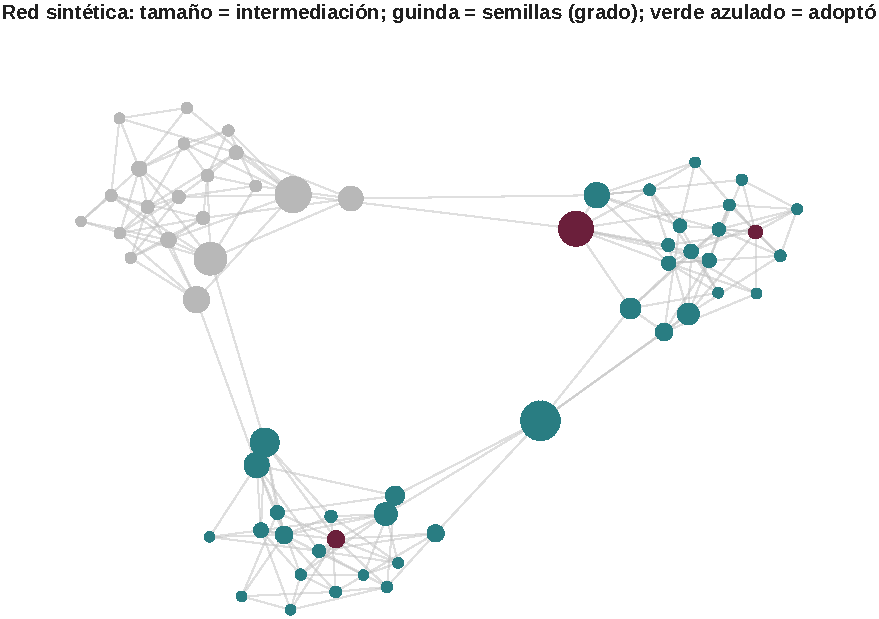
\includegraphics[width=\linewidth,height=0.66\textheight,keepaspectratio]{cap08_red_influencia.pdf}
\end{center}
\fuente{elaboración propia, MATLAB, red sintética, \texttt{rng(42)}.}
\end{frame}

\begin{frame}{Salida: seguidores no es influencia}
\begin{center}
  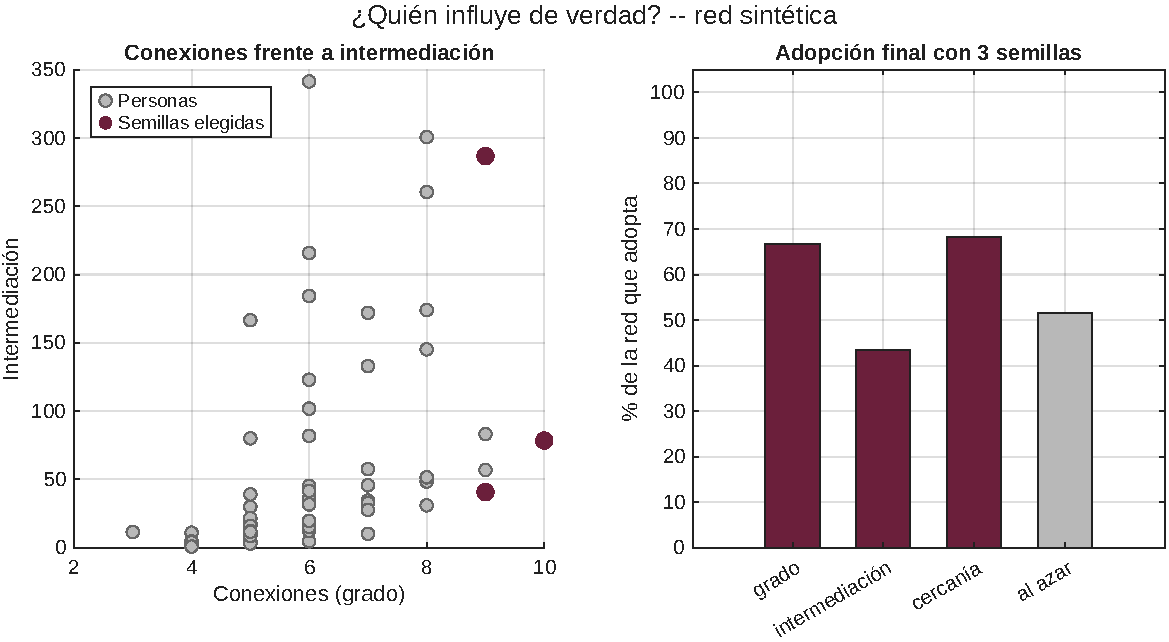
\includegraphics[width=\linewidth,height=0.62\textheight,keepaspectratio]{cap08_seguidores_vs_influencia.pdf}
\end{center}
\vspace{-4pt}
\begin{center}
  \small Top-5 por grado y por intermediación: coinciden en \textbf{1 de 5}. Adopción: grado \textbf{66.7\,\%}, intermediación \textbf{43.3\,\%}, azar \textbf{51.5\,\%}.
\end{center}
\fuente{elaboración propia, MATLAB, datos sintéticos.}
\end{frame}

\begin{frame}{Interpretación de negocio}
\begin{columns}[c]
  \column{0.48\textwidth}
  \begin{block}{Lo que muestran los datos}
    \small Los \textbf{puentes} no son los más conectados. Y elegir semillas por intermediación rindió \textbf{menos que el azar}.
  \end{block}
  \begin{alertblock}{Explicación probable}
    \small Un modelo de umbral exige \textbf{varios} contactos adoptantes; una persona-puente tiene pocos contactos \textbf{dentro} de cada grupo.
  \end{alertblock}
  \column{0.48\textwidth}
  \begin{exampleblock}{La medida depende del mecanismo}
    \small Para difundir \textbf{información simple}, los puentes ayudan. Para decisiones que exigen \textbf{validación social}, pesan los contactos densos. Es una red sintética: se aprende el \textbf{método de comparación}, no un orden universal.
  \end{exampleblock}
\end{columns}
\end{frame}

\begin{frame}{Ejercicio propuesto: tres corridas}
\begin{columns}[T]
  \column{0.52\textwidth}
  \begin{exampleblock}{Casos (solo el bloque de parámetros)}
    \scriptsize
    \begin{itemize}
      \item[\textbf{A}] Valores por defecto.
      \item[\textbf{B}] \textbf{Más puentes}: \texttt{pEntre} de 0.01 a 0.06.
      \item[\textbf{C}] \textbf{Grupos más densos}: \texttt{pEntre} en 0.01 y \texttt{pDentro} de 0.20 a 0.35.
    \end{itemize}
  \end{exampleblock}
  \column{0.44\textwidth}
  \scriptsize
  \begin{tabular}{@{}lccccc@{}}
    \toprule
    Caso & Con. & Coin. & Grado & Inter. & Azar \\
    \midrule
    A & \rule{0.45cm}{0.4pt} & \rule{0.45cm}{0.4pt} & \rule{0.45cm}{0.4pt} & \rule{0.45cm}{0.4pt} & \rule{0.45cm}{0.4pt} \\[2pt]
    B & \rule{0.45cm}{0.4pt} & \rule{0.45cm}{0.4pt} & \rule{0.45cm}{0.4pt} & \rule{0.45cm}{0.4pt} & \rule{0.45cm}{0.4pt} \\[2pt]
    C & \rule{0.45cm}{0.4pt} & \rule{0.45cm}{0.4pt} & \rule{0.45cm}{0.4pt} & \rule{0.45cm}{0.4pt} & \rule{0.45cm}{0.4pt} \\
    \bottomrule
  \end{tabular}\\[2pt]
  {\tiny Con.: conexiones. Coin.: coincidencias de 5. Grado/Inter./Azar: \% de adopción.}
\end{columns}
\vspace{2pt}
\begin{block}{Respondan con sus corridas}
  \scriptsize
  \begin{enumerate}
    \item Caso B: ¿qué ocurre con la adopción con semillas centrales y con las del azar? ¿Qué papel juegan los puentes?
    \item Caso C: ¿por qué una red más densa \textbf{dificulta} la cascada con el mismo umbral?
    \item ¿Por qué no basta con contratar a quien tiene más seguidores?
  \end{enumerate}
\end{block}
\end{frame}

\begin{frame}{Tercer insumo de la práctica «Recorrido del consumidor digital»}
\begin{columns}[T]
  \column{0.54\textwidth}
  \begin{block}{Sobre el caso de su equipo}
    \small Hoy agregan al entregable único las \textbf{figuras participantes} de su caso: quién ocupa cada uno de los siete papeles y \textbf{qué dato deja}.
  \end{block}
  \column{0.42\textwidth}
  \begin{exampleblock}{También entregan}
    \scriptsize
    \begin{itemize}
      \item El \textit{buyer persona} que usaría la organización del caso.
      \item Tres \textbf{limitaciones} del arquetipo frente a clientes reales.
    \end{itemize}
  \end{exampleblock}
\end{columns}
\end{frame}

\begin{frame}{Práctica con sus propios datos: app HTML}
\begin{columns}[T]
  \column{0.54\textwidth}
  \begin{block}{\texttt{cap08\_red\_datos\_propios.html}}
    \small Sin MATLAB y sin conexión: suban un Excel con \textbf{sus datos} y recorran 4 pasos:
    \scriptsize
    \begin{enumerate}
      \item Su red: componentes y conexiones.
      \item Centralidad: ¿quién es puente y quién tiene más contactos?
      \item La cascada: ¿a quién regalar el producto primero?
      \item Lectura de negocio y descarga en Excel.
    \end{enumerate}
  \end{block}
  \column{0.42\textwidth}
  \begin{exampleblock}{Reglas del archivo}
    \scriptsize
    \begin{itemize}
      \item Hoja \texttt{Conexiones}: \texttt{Persona\_A} y \texttt{Persona\_B}; de 10 a 150 personas.
      \item Hoja \texttt{Personas} (opcional): \texttt{Persona} y \texttt{Grupo}.
      \item \textbf{Seudónimos}, no nombres: una red expone a terceros.
      \item Sus datos \textbf{no salen} de su computadora.
    \end{itemize}
  \end{exampleblock}
\end{columns}
\end{frame}

\begin{frame}{Ética: un grafo expone a terceros}
\begin{alertblock}{Quien aparece como contacto de otra persona no consintió ser analizado}
  Una red de relaciones revela más que los datos de cada persona. Elegir semillas por centralidad significa \textbf{tratar distinto a quienes ocupan posiciones clave, sin que lo sepan}.
\end{alertblock}
\begin{block}{Como mínimo}
  \begin{itemize}
    \item La credibilidad que se compra es la que la audiencia cree \textbf{gratuita}: identificar el contenido pagado.
    \item Antes de mapear una red real: ¿\textbf{quién queda expuesto}, con qué \textbf{base legal} (Sesión 3) y para qué decisión?
  \end{itemize}
\end{block}
\end{frame}

%------------------------------------------------
\section[Caso]{Estudio de caso}
%------------------------------------------------

\begin{frame}{Caso: la marca de cosméticos}
\begin{exampleblock}{Caso ficticio}
  Presupuesto de lanzamiento. La agencia propone \textbf{una macroinfluenciadora} con dos millones de seguidores, o repartir el presupuesto entre \textbf{doce microinfluenciadoras} (20 a 50 mil) de seis comunidades de aficionados. La agencia sugiere la primera \enquote{por alcance}.
\end{exampleblock}
\begin{alertblock}{Lo que descubre el analista}
  \small Con datos de grupos públicos reconstruye una red: las microinfluenciadoras \textbf{conectan comunidades que apenas se tocan}; la macro pertenece a \textbf{una sola} comunidad grande.
\end{alertblock}
\end{frame}

\begin{frame}{Preguntas guía}
\small
\begin{enumerate}
  \item ¿Qué \textbf{medida de centralidad} ayudaría a decidir entre ambas opciones y por qué?
  \vspace{3pt}
  \item Si el producto exige \textbf{validación social} antes de comprar, ¿qué dice el laboratorio sobre elegir semillas por grado o por intermediación?
  \vspace{3pt}
  \item ¿Qué datos debería pedir la marca a cada influenciadora y qué \textbf{obligaciones de transparencia} aplican?
  \vspace{3pt}
  \item ¿Qué riesgos éticos tiene reconstruir la red a partir de grupos públicos?
\end{enumerate}
\begin{alertblock}{Entregable}
  \small Solución escrita con las cuatro preguntas respondidas.
\end{alertblock}
\end{frame}

%------------------------------------------------
\section{Cierre}
%------------------------------------------------

\begin{frame}{Síntesis: papeles, no personas}
\begin{itemize}
  \small
  \item Siete figuras: \textbf{usuario, consumidor, prosumidor, influenciador, decisor, comprador y evaluador}. Cada una deja un dato distinto.
  \item El \textit{buyer persona} es un \textbf{arquetipo de diseño}; sustituirlo con modelos de lenguaje es hoy \textbf{exploratorio}.
  \item El influenciador no se mide por seguidores: depende de \textbf{credibilidad, posición en la red y mecanismo de contagio}.
  \item El evaluador puede ser un \textbf{sistema}: la regla de decisión se vuelve una pregunta de diseño y de responsabilidad.
\end{itemize}
\vspace{4pt}
\begin{alertblock}{La regla de la sesión}
  \small Antes de contratar a quien tiene más seguidores, pregunten: \textbf{¿a quién escuchan, de verdad, quienes van a decidir?}
\end{alertblock}
\end{frame}

\begin{frame}{Autoevaluación rápida}
\footnotesize
\begin{enumerate}
  \item El término \enquote{prosumidor} fue acuñado por:
  \begin{itemize}
    \item[a)] Cooper (1999) en diseño de software;
    \item[b)] \alt<2->{\textcolor{IPNguinda}{\textbf{Toffler (1980), en \textit{The Third Wave}}}}{Toffler (1980), en \textit{The Third Wave}};
    \item[c)] PROFECO (2023).
  \end{itemize}
  \item La persona-puente se distingue de la más conectada porque:
  \begin{itemize}
    \item[a)] siempre tiene más seguidores;
    \item[b)] \alt<2->{\textcolor{IPNguinda}{\textbf{tiene alta intermediación: muchos caminos entre grupos pasan por ella}}}{tiene alta intermediación: muchos caminos entre grupos pasan por ella};
    \item[c)] no pertenece a ningún grupo.
  \end{itemize}
  \item La Guía de Publicidad para Influencers de PROFECO es:
  \begin{itemize}
    \item[a)] una ley específica con régimen sancionador propio;
    \item[b)] \alt<2->{\textcolor{IPNguinda}{\textbf{una guía de recomendaciones con fundamento en la LFPC}}}{una guía de recomendaciones con fundamento en la LFPC};
    \item[c)] un estándar internacional.
  \end{itemize}
\end{enumerate}
\end{frame}


\begin{frame}{Evidencias del portafolio}
\begin{block}{Pasos para subir los trabajos al portafolio}
    \begin{itemize}
    \item Accede a esta carpeta de evidencia: \url{https://drive.google.com/drive/folders/1sr_SAVkl_Mjil6ZRWz3O2mveMoZVW6cp?usp=sharing}
    \item Crea una carpeta con tu nombre y organiza en ella todos tus entregables del semestre.
    \item Considera los tiempos límite establecidos para cada actividad.
    \end{itemize}
  \end{block}
\end{frame}


\begin{frame}{Evidencias del portafolio}
\small
\begin{columns}[T]
  \column{0.48\textwidth}
  \begin{block}{Infografía colaborativa}
    \scriptsize Las siete figuras participantes del caso real: quién ocupa cada papel y qué dato deja.
  \end{block}
  \begin{block}{Reporte de investigación}
    \scriptsize \textit{Buyer persona} de la organización del caso y tres limitaciones frente a clientes reales.
  \end{block}
  \column{0.48\textwidth}
  \begin{block}{Solución de casos}
    \scriptsize Caso de la marca de cosméticos, cuatro preguntas por escrito.
  \end{block}
  \begin{block}{Reporte de práctica}
    \scriptsize Cuadro de los casos A, B y C con las respuestas. Se integra al entregable único de «Recorrido del consumidor digital».
  \end{block}
\end{columns}
\end{frame}

\begin{frame}{Aprendizaje autónomo}
\footnotesize
\begin{enumerate}
  \item Ejecutar \texttt{cap08\_red\_influencia\_\allowbreak interactivo.html}, completar el cuadro de los \textbf{casos A, B y C} y comparar los tres criterios de semilla con el \textbf{histograma de los 100 sorteos al azar}.
  \vspace{1pt}
  \item Anotar en \textbf{dos líneas} por qué una sola muestra aleatoria no sirve como referencia.
  \vspace{1pt}
  \item (Opcional) Con \texttt{cap08\_red\_datos\_propios.html} (opcional), cargar el \textbf{Ejemplo 2} (club de aficionados) y comparar qué criterio de semillas rinde más.
\end{enumerate}
\vspace{2pt}
\begin{alertblock}{Fecha de entrega}
  En la fecha acordada en clase, en su carpeta del portafolio.
\end{alertblock}
\end{frame}

\begin{frame}{Glosario de la sesión}
\scriptsize
\begin{description}
  \item[Prosumidor] Persona que consume y produce (Toffler, 1980).
  \item[Grado] Número de conexiones de una persona.
  \item[Intermediación] Fracción de los caminos más cortos entre otros pares que pasa por una persona.
  \item[Cercanía] Inverso de la distancia media a todos los demás.
  \item[Cascada por umbral] Cada persona adopta cuando al menos una fracción de sus contactos ya adoptó.
  \item[Semilla] Persona que adopta en la ronda 0 (\texttt{nSemillas}: entero de 1 a 10).
  \item[\texttt{pDentro} / \texttt{pEntre}] Probabilidad de conocerse dentro del grupo (0.05 a 0.50) / entre grupos (0 a 0.10).
  \item[\texttt{umbral}] Fracción de contactos que deben haber adoptado (0.05 a 0.90).
\end{description}
\end{frame}

\begin{frame}{Referencias}
\tiny
\begin{itemize}
  \item[] Argyle, L. P., Busby, E. C., Fulda, N., Gubler, J. R., Rytting, C. y Wingate, D. (2023). Out of one, many: Using language models to simulate human samples. \textit{Political Analysis}. \url{https://doi.org/10.1017/pan.2023.2}
  \item[] Barari, M., Eisend, M. y Prasad Jain, S. (2025). A meta-analysis of the effectiveness of social media influencers. \textit{Journal of the Academy of Marketing Science}. \url{https://doi.org/10.1007/s11747-025-01107-3}
  \item[] Bisbee, J., Clinton, J. D., Dorff, C., Kenkel, B. y Larson, J. M. (2024). Synthetic replacements for human survey data? The perils of large language models. \textit{Political Analysis, 32}, 401--416. \url{https://doi.org/10.1017/pan.2024.5}
  \item[] Brandes, U. (2001). A faster algorithm for betweenness centrality. \textit{Journal of Mathematical Sociology, 25}(2), 163--177. \url{https://doi.org/10.1080/0022250X.2001.9990249}
  \item[] Cooper, A. (1999). \textit{The inmates are running the asylum}. SAMS/Macmillan.
  \item[] Granovetter, M. (1978). Threshold models of collective behavior. \textit{American Journal of Sociology, 83}(6), 1420--1443.
  \item[] Instituto Nacional de Estadística y Geografía. (2026). \textit{ENDUTIH 2025} (Comunicado de prensa 32/26). INEGI.
  \item[] Leung, F. F., Gu, F. F., Li, Y., Zhang, J. Z. y Palmatier, R. W. (2022). Influencer marketing effectiveness. \textit{Journal of Marketing, 86}(6), 93--115. \url{https://doi.org/10.1177/00222429221102889}
  \item[] Procuraduría Federal del Consumidor. (2023). \textit{Guía de Publicidad para Influencers}. DOF. \url{https://dof.gob.mx/2023/PROFECO/guiainfluencers.pdf}
  \item[] Toffler, A. (1980). \textit{The third wave}. William Morrow.
  \item[] Webster, F. E. y Wind, Y. (1972). A general model for understanding organizational buying behavior. \textit{Journal of Marketing, 36}(2), 12--19.
\end{itemize}
\end{frame}

\begin{frame}
    \begin{center}
        {\Large \textcolor{IPNguinda}{\textbf{Gracias}}}\\[6pt]
        {\color{IPNdorado}\rule{0.4\linewidth}{1.2pt}}\\[6pt]
        Dr. Aboud Barsekh-Onji \\
        \small Instituto Politécnico Nacional · ESCA Unidad Santo Tomás \\
        \small \texttt{ORCID: \href{https://orcid.org/0009-0004-5440-8092}{0009-0004-5440-8092}}
    \end{center}
\end{frame}

\end{document}
